%!TEX root = ../main.tex
% Chapter Template


\chapter{Preliminaries and Notation} % Main chapter title
\label{ch:Preliminaries} % Change X to a consecutive number; for referencing this chapter elsewhere, use \ref{ChapterX}

\todo[inline]{This section has content which I did not develop, but that I use. The content I developed follows in the next chapters.}

%----------------------------------------------------------------------------------------
%	SECTION 1
%----------------------------------------------------------------------------------------
\section{Notation and Constructions on Sets and Functions}
\subsection{Sets and elements}
We denote \emph{sets} by upper-case letters $X,Y,Z,$ etc, and we denote their \emph{elements} by lower-case letters $x, y, z, $ etc. 

We denote the set of natural numbers by $\mathbb{N}$ and the set of natural numbers without zero by $\mathbb{N}^+$. Similarly, we denote the set of real numbers by $\mathbb{R}$ and the set of positive real numbers (excluding zero) by $\mathbb{R}^+$.

We denote the size of a finite set $X$ by $|X|$, and the empty set by $\emptyset$.

\subsection{Functions}
We denote \emph{functions} by lower-case letters $f,g,h,$ etc. A function $f\colon X\rightarrow Y$ maps the elements from the set $X$ to elements of the set $Y$. An \emph{endofunction} is a function $g\colon X\rightarrow X$ which maps a set $X$ to itself. We denote function composition by $\circ$. 
We say that an endofunction $h\colon X \rightarrow X$ has finite support iff $h(x)\neq x$ for a finite number of $x$ in $X$, even if $X$ is infinite.

\subsection{Range set}
A \emph{range set} $n$ where $n\in \mathbb{N}^+$ is a set of $n$ elements, i.e., $n=\set{0,1, \ldots, n-1}$. It is usually clear from the context when $n$ represents a number or a range set. We highlight three important range sets: 0, 1 and 2.

The range set 0 is equal to the empty set $\emptyset$. 
The range set 1, which is equal to the set $\set{0}$, serves as a constant for several set operations (modulo isomorphism).
The range set 2, which is equal to $\set{0,1}$, to model booleans: 0 models $\false$ and $1$ models $\true$. 

\subsection{Subsets $X\rightarrow 2$}
Given a set $X$, we characterise the \emph{subsets of $X$} using functions of type $X\rightarrow 2$; we say that $x\in X$ is an element of the subset characterised by $f\colon X\rightarrow 2$ iff $f(x)=1$. 
 
\subsection{Exponential Set $Y^X$}
The \emph{exponential set} $Y^X$ is the set of all functions of type $X\rightarrow Y$. 
The exponential set $1\rightarrow X$ is isomorphic to $X$, and we use it to select objects from $X$; more precisely, we choose an element $x\in X$ via a function $f\colon 1\rightarrow X$ such that $f(0)=x$. (This seems overcomplicated at first, but we use this equivalence when discussing the following concepts of $F$-algebra and $F$-coalgebra.)

\subsection{Sum Set $X+Y$}
The \emph{sum set} $X + Y$ is the disjoint union of $X$ and $Y$, i.e. 
\begin{align*}
    X + Y\triangleq\set{ \iota_1(x) |x\in X} \cup \set{\iota_2(y) | y\in Y},
\end{align*}
where $\iota_1$ and $\iota_2$ act as different tags.
\subsection{Product Set $X\times Y$}
The \emph{product set} $X\times Y$ is the cartesian product of $X$ and $Y$, i.e. 
\begin{align*}
    X\times Y\triangleq\set{(x,y)|x\in X, y\in Y}.
\end{align*}
The \emph{finite product set} of sets $X_1, \ldots, X_n$ is their cartesian product; i.e., $X_1\times \ldots \times X_n$. We denote product sets by upper-case letters with an arrow above $\vec{X},\vec{Y}, \vec{Z}$, etc.
\subsection{Vector/Tuple $\vec{x}$}
Given a finite product set $\vec{X}=X_1\times \ldots \times X_n$, we denote the elements of $\vec{X}$ by $\vec{x}$, $\vec{y}$, $\vec{z}$, etc. We call these elements \emph{vectors} or, alternatively, \emph{tuples}. 

\subsection{Coordinates $\vec{x}[\pi]$}
Given a finite product set $\vec{X}=X_1\times \ldots \times X_n$, its \emph{coordinates} are $\pi_1, \ldots, \pi_n$, where $\pi_i\colon \vec{X} \rightarrow X_i$ extract the $i$-th value of a vector; i.e., $\pi_i(x_1, \ldots, x_n)\triangleq x_i$, for $1\leq i \leq n$. We often write the expression $\vec{x}[\pi]$ instead of $\pi(\vec{x})$ when $\pi$ is a coordinate. %We sometimes use the alternative notation $\vec{x}_\pi$ to denote $\vec{x}[\pi]$, usually when $\pi$ is a natural number.

We use natural numbers for coordinates when no explicit set of coordinates is provided. More precisely, given $\vec{x}\in X_1\times \ldots \times X_n$ where $\vec{x}=(v_1, \ldots, v_n)$, if no set of coordinates is provided, then we use the coordinates $1, 2, \ldots , n$, so $\vec{x}[i]=v_i$ for $i\in \set{1, \ldots, n}$. 

\subsection{Constant Function $\Delta_x$}
Given sets $X$ and $Y$, each element $x\in X$ lifts to a \emph{constant function} $\Delta_x\colon Y\rightarrow X$, defined by $\Delta_x(y)=x$, for $y\in Y$.

\subsection{Pair Function $(f,g)$}
Given two functions $f\colon X\rightarrow Y$ and $g\colon X\rightarrow Z$, the \emph{pair function} $(f,g)\colon X\rightarrow Y\times Z$ is defined by $(f,g)(x)=(f(x),g(x))$.

\subsection{Product Function $f\times g$}
Given two functions $f\colon X\rightarrow Y$ and $g\colon A\rightarrow B$, the \emph{product function} $f\times g\colon X\times A\rightarrow Y\times B$ is defined by $f\times g(x,a)=(f(x),g(a))$.

\subsection{Function Mapping $f(X)$}
Given a set $X$ and a function $f\colon X\rightarrow Y$, the \emph{mapping of $f$ over $X$}, denoted $f(X)$, is the set defined by $f(X)\triangleq\set{f(x)| x\in X}$.

\section{Category Theory Preliminaries and Notation}

\subsection{Categories, Objects and Arrows}
A \emph{category} $\AsCategory{C}$ is a mathematical concept similar to a graph, comprised of two aspects: a collection of \emph{objects}, denoted $Obj(\AsCategory{C})$, and a collection of \emph{arrows} among those objects, denoted $Arr(\AsCategory{C})$. Each category satisfies the following  rules:
\begin{itemize}
    \item every object $X$ has an identity arrow that maps $X$ to itself, denoted $\id_X$,
    \item given the objects $X, Y$ and $Z$, and the arrows $X\xrightarrow{f}Y$ and $Y\xrightarrow{g}Z$, the arrow $X\xrightarrow{g\circ f}Z$ exists; i.e. the composition of arrows is well defined,
    \item the identity arrows act as units for arrow composition; i.e., for $X\xrightarrow{f}Y$, the equality $\id_{Y}\circ f=f=f\circ \id_{X}$ holds.
    \item the composition of arrows is associative; i.e., $(h\circ g)\circ f = h \circ (g\circ f)$.
\end{itemize}

\subsection{Commutative Diagram}
A \emph{commutative diagram} is a directed graph which visually represents equations. Like any directed graph, source nodes do not have incoming arrows, and sink nodes do not have outgoing arrows, and they represent the beginning and end of equations. For example, given the functions $f\colon X\rightarrow Y$, $g\colon Y\rightarrow Z$ and $h\colon Z\rightarrow A$, the equalities $(h\circ g)\circ f= h\circ g \circ f= h \circ (g\circ f)$ is represented by the diagram shown in Figure~\ref{fig:Preliminaries:CommutativeDiagram}.

\begin{figure}[t] 
    \centering
    \begin{tikzcd}[column sep=1.5cm, row sep=1.5cm]
         X
            \arrow[r,"f"]
            \arrow[rr,bend left, "g\circ f"]
            %\arrow[r,"c"]
            %\arrow[d,"1"']
        &Y
            \arrow[r,"g"]
            \arrow[rr,bend right, "h\circ g"]
        &Z
            \arrow[r,"h"]
        &A
            %\arrow[u,"1^{-1}"']
    \end{tikzcd}
    \caption{Commutative diagram describing the equality $(h\circ g)\circ f= h\circ g \circ f= h \circ (g\circ f)$}
    \label{fig:Preliminaries:CommutativeDiagram} 
\end{figure}
\subsection{Initial and Terminal Objects}
A category $\AsCategory{C}$ has an \emph{initial object}, often denoted by 0, if there exists a unique arrow from $0$ to every object $o$ in the category. Dually, a category $\AsCategory{C}$ has a \emph{final object}, often denoted by 1, if there exists a unique arrow from every object $o$ in the category to 1. 

A category may have several different initial and terminal objects, but they are always unique modulo isomorphism.

\subsection{Functor}
Functors are to categories what arrows are to objects. A \emph{functor} $F$ maps a category $\AsCategory{C}$ to a category $\AsCategory{D}$, mapping $Obj(\AsCategory{C})$ to $Obj(\AsCategory{D})$, and $Arr(\AsCategory{C})$ to $Arr(\AsCategory{D})$ such that the following conditions are satisfied for all objects $X, Y, Z$ and arrows $f,g$.
\begin{itemize}
    \item for $f\colon X\rightarrow Y$, $f$ is mapped to a function of type $g\colon F(X)\rightarrow F(Y)$,
    \item $\id_X$ is mapped to $\id_{F(X)}$; i.e. $F(\id_{X})=\id_{F(X)}$.
    \item if $f\colon X\rightarrow Y$ and $g\colon Y\rightarrow Z$, then $F(g\circ f)=F(g)\circ F(f)$.
\end{itemize}
These conditions ensure functors preserve the structure of the category they are mapping.

\section{The Category of Sets and Functions}
The \emph{category of sets and functions} $\AsCategory{Set}$ is the category whose objects are sets and whose arrows are functions. The empty set $0$ is the initial object, and any set isomorphic to the range set 1 is a terminal object.

\subsection{Currying}
\emph{Currying} is the use of the isomorphism between the sets $Z^{X\times Y}$ and $Z^{Y^X}$ which maps a function $f\colon (X\times Y)\rightarrow Z$ to a function $g\colon X\rightarrow Z^Y$ such that $g(x)(y)=f(x,y)$ for $x\in X$ and $y\in Y$. We use currying to adjust the types between equivalent constructions (e.g. between Automata and $F$-coalgebras).

\subsection{Partial Application}
Given a function $f\colon X\rightarrow Y \rightarrow Z$ and $x\in X$, the \emph{partial application} of $f$ given $x$ is the function $f_x\colon Y \rightarrow Z$, defined for $y\in Y$ by $f_x(y)=f(x)(y)$.

\subsection{Monoids and Sequences} 
A \emph{monoid} in the category $\AsCategory{Set}$ is a set $X$ paired with a sum function $+\colon X\rightarrow X\rightarrow X$ and a unit element $0\in X$ such that $0$ is neutral for $+$ and $+$ is associative. 

We highlight two monoids for a given set $X$: the \emph{free monoid of $X$} and the \emph{endofunctions monoid of $X$}.

The \emph{free monoid of $X$} is the set $X^*$ of finite sequences of elements of $X$, where the sum function is sequence concatenation $\cdot$ and the unit is the empty sequence $\varepsilon$.

The \emph{endofunctions monoid of $X$} is the set $X^X$ of endofunctions in $X$, where the sum is function composition $\circ$ and the unit is the identity function $\id_X$.

\subsection{Languages}
Given a set $X$, a \emph{language with alphabet $X$} is a subset of $X^*$. 

\subsection{Deterministic Finite Automata (DFA)}
Given a finite set $A$, a \emph{deterministic finite automaton} (DFA) is a tuple $\mathbb{X}=(X,x_0,\delta,F)$, where $X$ is a finite set, $x_0$ is an element of $X$, $\delta\colon X\times A \rightarrow X$ is a transition function, and $F\colon X\rightarrow 2$ is a subset of $X$ which marks accepting states. Given a sequence $w\in A^*$, we say that the automaton $\mathbb{X}$ \emph{accepts} $w$ if and only if the following conditions are satisfied,
\begin{itemize}
    \item if $w=\varepsilon$, then $\mathbb{X}$ accepts $w$ iff $F(x_0)=1$, 
    \item if $w=a\cdot w'$, then $\mathbb{X}$ accepts $w$ iff the automaton $(X,\delta(x_0,a),\delta,F)$ accepts $w'$, with $a\in A$ and $w'\in A^*$.
\end{itemize}
The denotational semantics of a DFA is the language with alphabet $A$ whose sequences it accepts, rejecting the rest.

\subsection{Set Isomorphisms}
\todo[inline]{Homomorphisms and isomorphisms}
\subsubsection{List of Relevant Isomorphisms}
\begin{itemize}
    \item $1\times X \simeq X$,
    \item $2\times X\simeq X+X$,
    \item $X^1\simeq X$,
    \item $X^2\simeq X\times X$,
    \item $Z^{X\times Y}\simeq Z^{Y^X}$,
    \item $X\times Y \simeq Y\times X$
    \item $X + Y \simeq Y+ X$
    \item $|X|=n$ iff $X\simeq n$.
    \item $\underbrace{\left(X\times\ldots\times X\right)}_\text{$n$ times}\simeq X^n$ (for this case, we say that $n$ is the set of coordinates of $X^n$)
\end{itemize}
\section{Universal (Co)Algebra Preliminaries and Notation}
\label{sec:Preliminaries:Coalgebras}
% \todo[inline]{ntroduction to the world of (co)algebras and explain why you want to use them. They are a wonderful way to unify the formalism of the thesis.}
% \todo[inline]{Complete here}
%\todo[inline]{*Puts an Edna Mode face* NO MONADS (unless necessary)}
%\subsection{$\Monad$-algebras, $\Functor$-coalgebras and $\lambda$-bialgebras}
\subsection{$F$-(co)algebras}
Given an endofunctor $F$ in a category $\AsCategory{C}$, an \emph{$F$-coalgebra} is a pair $(X,X\xrightarrow{c}F(X))$ of an object $X$ and a morphism $c\colon X\rightarrow F(X)$. We use $F$-coalgebras to model dynamic systems with state. We call $X$ the \emph{carrier} and $c$ the \emph{dynamics}.

Dually, an \emph{$F$-algebra} is a pair $(X,F(X)\xrightarrow{a}X)$.

\subsection{Pointed coalgebras}
Pointed coalgebras are coalgebras with a distinguished state, usually referred to as the \emph{initial state}. Formally, for a functor $F$, a pointed $F$-coalgebra is a triple $(X,c, x_0)$ where $(X,c)$ is an $F$-coalgebra and $(X, x_0)$ is a $\Delta_X$-algebra, i.e., $x_0\colon 1\rightarrow X$, and $x_0(\star)$ characterises the initial state.

\subsection{Automata as Pointed Coalgebras}
DFA which characterise languages with an alphabet $A$ can be modelled by coalgebras of the functor $F(X)=2\times X^A$. Given a DFA $(X,x_0,\delta,F)$, the corresponding $F$-coalgebra is $(X,(F,\delta))$, where $(F,\delta)\colon X\rightarrow 2\times X^2$ is a function pair. We can make this coalgebra pointed by adding a function $x_0\colon 1\rightarrow X$ to mark the initial state.

In general, given sets $I$ and $O$, we can model transition systems whose denotational semantics are functions of type $I^*\rightarrow O$; i.e., systems which process a finite sequence of elements in $I$ and respond with an element in $O$. The corresponding functor in this case is $F(X)=O\times X^I$. An $F-$coalgebra would be of the form $(X,X\xrightarrow{(\gamma,\delta)}O\times X^I)$, with $\gamma\colon X\rightarrow O$ and $\delta\colon X\rightarrow X^I$; the function $o$ lets us explore the component in the state $x$, and $\delta$ lets us perform transitions. We write $x/o$ to denote $\gamma(x)=o$, and we write $x^i$ as a shorthand for $\delta(x)(i)$. 

% \subsection{States and Components}
% We often use vectors/tuples as a states. We access the values inside states by means of projection functions. If the carrier is a product set $\vec{X}=Y_1 \times\ldots Y_n$, we can use, for $j=1..n$, the projection functions $\pi_j\colon \vec{X}\rightarrow Y_j$ defined, for $\vec{x}=(v_1,\ldots,v_n)$, by $\pi_j(\vec{x})\triangleq v_j$. In this case, we say that $\pi_1$ to $\pi_n$ are the \emph{components} of $\vec{X}$ and its elements. Since both coalgebras and components are functions from the carrier, we use bracket notation for component to distinguish them, i.e., we write $\vec{x}[\pi_j]$ instead of $\pi_j(\vec{x})$.  %, or, alternatively the \emph{state variables} of states in $X$. 
% Whenever we write a state or a carrier  with arrows above them (i.e., $\vec{x}$ or $\vec{X}$), we imply that they have more than one component. Note that if the carrier $X$ has only one component, then it must be the identity function $\id\colon X\rightarrow X$. 
% \todo[inline]{Consider $\vec{x}.\pi_j$ too, called dot notation}
%A \emph{$\Monad$-algebra} for a monad $\Monad=(\MFunctor,\eta,\mu)$ is a pair $(\TheSet,\Monad(\TheSet)\xrightarrow{a}\TheSet)$ of an object $\TheSet$ and a morphism $a\colon \Monad(\TheSet)\rightarrow\TheSet$ which, due to the relationship between monads and adjunctions, satisfies two properties: the \emph{multiplication square} and the \emph{unit triangle}, shown in Figure~\ref{fig:MultiplicationSquare}.
%
%%\subsubsection The compositions $a\circ \mu_X$ and $a\circ T(a)$ are equal.
%\begin{figure}[h]
%\centering
%\begin{minipage}{0.45\textwidth}
% \centering
%\begin{tikzcd}
%    T^2(X) \arrow{r}{T(a)} \arrow[swap]{d}{\mu_X} & T(X) \arrow{d}{a} \\
%    T(X) \arrow{r}{a}& X
% \end{tikzcd}
%\end{minipage}
% \begin{minipage}{0.45\textwidth}
% \centering
%\begin{tikzcd}
%    T(X) \arrow{r}{a} \arrow[swap]{dr}{1_{T(X)}} & X\arrow{d}{\eta} \\
%    & T(X)
%  \end{tikzcd}
%  \end{minipage}
%  \caption{Multiplication square (left) and unit triangle (right).}
%\label{fig:MultiplicationSquare}
%\end{figure}
%Given a state structure $S$, we can use the State monad .
%\begin{align}
%State_S(X) = (S\times X)^S 
%\end{align}
%
%\begin{align}
%\eta_X:X\rightarrow  (S\times X)^S\\
%\eta_X(x)= \lambda s \rightarrow (s,x)
%\end{align}
%
%%\begin{align}
%%>>=\colon  (S\rightarrow (T,S))\rightarrow (T\rightarrow (S\rightarrow (Y,S)) \rightarrow  (S\rightarrow (Y,S))\\
%%m >>= f = \lambda s \rightarrow \text{let $(t,s')=m(s)$ in $f(t)(s')$} 
%%\end{align}
%
%\begin{align}
%\mu_X:(S\times (S\times X)^S)^S\rightarrow  (S\times X)^S\\
%\mu_X(\mathbf{x})= \lambda s \rightarrow \text{let $(s',f)=\mathbf{x}(s)$ in f(s')}
%\end{align}
%\todo[inline]{THERE IS NO NEED FOR MONADS AT THE MOMENT. Monads seem to be what maps a type $X$ to an initial/final $F$-coalgebra of a functor where $X$ is constant}
%\subsection{An Intuition of States and Time}
%\subsection{Catamorphisms, Anamorphisms, Final and Initial $F$-Coalgebras}
\subsection{The Category of $F$-coalgebras and $F$-homomorphisms}
Given a functor $F$, the \emph{category of $F$-coalgebras}, denoted $\AsCategory{Coalg_F}$ is the category whose objects are $F$-coalgebras and whose arrows are \emph{$F$-homomorphisms}. An \emph{$F$-homomorphism} $\mathbb{X}\xrightarrow{f} \mathbb{Y}$ between an $F$-coalgebra $\mathbb{X}=(X,c)$ and an $F$-coalgebra $\mathbb{Y}=(Y,d)$ is a function $f\colon X\rightarrow Y$ such that
\begin{align}
    F(f)\circ c = d\circ f.
\end{align}

\subsection{Semantic Map and Final $F$-Coalgebras}
Let $F$ be a functor such that $F(X)=O\times (X)^I$, and let $I$ and $O$ be sets; we define the set $\sigma F\triangleq O^{I^*}$, and we define the function pair $(?, (\cdot)')\colon \sigma F\rightarrow O\times (\sigma F)^I$, for $\phi \in \sigma F$, $i\in I$ and $w\in I^*$, by
\begin{align}
    \phi? \triangleq \phi(\varepsilon),
    \phi'(i)(w) \triangleq \phi(i\cdot w)
\end{align}
Following convention, we write $\phi'(i)$ as $\phi^i$, and the pair $(?, (\cdot)')$ as $1_F$. The pair $(\sigma F, 1_F)$ is a \emph{final $F$-coalgebra}, since it is a final object in the category $\AsCategory{Coalg_F}$.

Given an $F$-coalgebra $(X,c)$ where $c=(\gamma,\delta)$, the unique $F$-homomorphism between $(X,c)$ and $(\sigma F, 1_F)$ is given by a function $!_c\colon X\rightarrow \sigma F$, which is defined for $x\in X$, $i\in I$ and $w\in I^*$ by 
\begin{align}
    !_c(x)(\varepsilon)\triangleq \gamma(x),\quad \text{and} \quad 
    !_c(x)(i\cdot w)\triangleq !_c(x^i)(w).
\end{align}
The function $!_c$ is called the \emph{semantic map} because it maps $x\in X$ to its denotational semantics in $\sigma F$. For example, in the case of DFA as coalgebras, it maps each state $x$ in the carrier of the coalgebra to the language it would be recognised if $x$ were the initial state in the DFA.

\subsection{Bisimilarity}
Given $F$-coalgebras $(X,c)$ and $(Y,d)$, we say that states \emph{$x\in X$ and $y\in Y$ are bisimilar}, denoted $x\sim y$, if and only if $!_c(x)=!_d(y)$. In other words, $x$ and $y$ are bisimilar iff they have the same semantics.

\subsection{Coalgebraic Specification Language}
Given a functor $F(X)=O\times X^I$ where $O$ and $I$ are fixed sets, a \emph{coalgebraic specification language} for $F$ is an $F$-coalgebra $(\mathcal{E},c)$ where $\mathcal{E}$ is a set of expressions whose semantics are given by the semantic map $!_c$.

For example, consider the functor $F(X)=2\times X^2$; we define the set of expressions $\mathcal{E}$ by the grammar
\begin{align}
    e::= ID:0?ID\land1?ID\land\downarrow (0|1)
\end{align}
where $ID$ is a set of identifiers. We define the pair function $c=(\gamma,\delta)\colon \mathcal{E}\rightarrow F(\mathcal{E})$ by 
\begin{align*}
    \gamma(x:0?\land1?z\land\downarrow a)&\triangleq a\\
    \delta(x:0?y\land1?z\land\downarrow a)(0)&\triangleq y\\
    \delta(x:0?y\land1?z\land\downarrow a)(1)&\triangleq z.
\end{align*}
The expression $x:0?x\land1?x\land\downarrow 1$ can be considered to describe a single-state automaton whose single state is  accepting, and it loops to itself on both inputs 0 and 1. The semantic map $!_c$ maps the expression $x:0?x\land1?x\land\downarrow 1$ to the language $2^*$.%, i.e., the language which contains every sequence in $2^*$.
\todo[inline]{Cite Kleene Coalgebra somehow}

\subsection{Completeness}
Given a coalgebraic specification language $L=(\mathcal{E},c)$ for the functor $F(X)=O\times X^I$, we say that $L$ is \emph{complete} if and only if the semantic map $!_c\colon \mathcal{E}\rightarrow \sigma F$ is surjective. In other words, for every behaviour $\phi\in \sigma F$, there exists an expression $e\in \mathcal{E}$ such that $!_c(e)=\phi$.

\subsection{Soundness}
Given a coalgebraic specification language $L=(\mathcal{E},c)$ for the functor $F(X)=O\times X^I$ and a notion of equivalence in $\mathcal{E}$ modelled by a function $\equiv \colon \mathcal{E}\times \mathcal{E}\rightarrow 2$, we say that $L$ is \emph{sound} if and only if, for $e_1, e_2\in \mathcal{E}$, if $e_1\equiv e_2$, then $e_1\sim e_2$; i.e., if two expressions are equivalent, then they have the same behaviour.

\section{Coinduction}
Coinduction is a dual principle to induction, and we use it to define what things are in terms of how they behave. 
\todo[inline]{I'll come back to this}

\subsection{Coinduction Proof Principle}
\todo[inline]{Coinductive Definitions?}
\subsection{Bisimulation}
% \section{Spectre}
% \label{sec:Preliminaries:Spectre}
% \todo[inline]{And Meltdown?}
% \subsection{Spectre V1}
% %\todo[inline]{}
% \subsection{Spectre V2}
\section{Attacker Classification via Latent-Behaviour Analysis}
\todo[inline]{This section may be better in its own chapter?}
\todo[inline]{Cite the sources that give these definitions. Get them from the chapter.}
\subsection{And-inverter Graphs (AIGs): Input, Latches, Gates, Components}
An \emph{And-inverter Graph} is a directed graph which models a system of equations \cite{AIGs,AIGs2}. AIGs describe hardware models at the bit-level \cite{AIGER}, and have attracted the attention of industry partners including IBM and Intel \cite{HWMCC2014BM}. 

Formally, an AIG has $m$ boolean 
inputs, $n$ boolean state variables and $o$ boolean gates. The elements in the set 
$W=\set{w_1, \ldots, w_m}$ represent the \emph{inputs}, the elements in 
$V=\set{v_1, \ldots, v_n}$ represent the \emph{latches}, and the elements in 
$G=\set{g_1, \ldots, g_o}$ represent the \emph{and-gates}. We assume that $W$, $V$ and $G$ are pairwise disjoint, and we define the set of \emph{components} $C$ by $C\triangleq W + V + G$. Without loss of generality, we assume that $W$, $V$ and $G$ are range sets.

\subsection{State and Input Vectors}
\label{sec:Preliminaries:AIGStates}
The \emph{states} of an AIG are all the different valuations of the variables in $V$.
Formally, a state $\vect{v}$ is a vector with coordinates in $V$ and values in $2$, so the set of all states is $\vec{V}=2^V$. This definition only considers latches to be part of the state; gates, inputs and requirements are external to the state.

Similarly, the \emph{input vector} is a
valuation of the variables in $W$. An input vector $\vect{w}$ is a vector with coordinates in $W$ and values in $2$; the set of input vectors is $\vec{W}=2^W$. 
% We refer to the set of all states by $\vect{V}%\triangleq\Bool^V
% $, and to the set of all inputs by $\vect{W}%\triangleq\Bool^W
% $. 
For  $t\in \Nat$, we denote the state of the system at time $t$ by $\vect{v}(t)$.
% with 
% %\begin{align*}
% $\vect{v}(t)\triangleq \AsSequence{v_1(t), \ldots, v_n(t)}$. %,g_1(t),\ldots,g_o(t));
% %\end{align*} 
The initial state is $\vect{v}(0)$. %, defined by the initial equations for the latches. 
Similarly, we denote the input of the system at time $t$ by $\vect{w}(t)$. %, with $\vect{w}(t)\triangleq\AsSequence{w_1(t), \ldots, w_n(t)}$. 
There are no restrictions or assumptions over the value of $\vect{w}(t)$.%, so it can take any value in $\vect{W}$ at every time $t$.

\subsection{Expressions}
An \emph{expression} $e$ is described by the grammar $e::= 0\ |\ 1\ |\ c\ |\ \lnot c$, where $c \in C$. The set of all expressions is $E$. We use AIG expressions to describe a system of equations over discrete time steps $t=0,1,..$. To each latch $v\in V$ we associate a transition {equation} of the form $v(t+1) = e(t)$ and an initial equation of the form $v(0)=b$, where $e\in E$ and $b\in \Bool$. To each gate $g\in G$ we associate an equation of the form $g(t)=e_1(t)\land e_2(t)$, where $e_1,e_2\in E$. 

\subsection{Invariant Requirements}
Given an expression $e\in E$, the \emph{invariant $\Always e$} is the property that requires $e(t)$ to be true for all $t\geq 0$. The system $S$ \emph{fails the invariant $\Always e$} iff there exists a finite sequence of inputs ${\vect{w}_0, \ldots, \vect{w}_t}$ such that, if $\vect{w}(i)=\vect{w}_i$ for $0\leq i \leq t$, then $e(t)$ is false. The system \emph{satisfies} the invariant $\Always e$ if no such sequence of inputs exists. Every expression $e$ represents a boolean predicate over the state of the latches of the system, and can be used to characterise states that are unsafe. These expressions are particularly useful in safety-critical hardware, as they can signal the proximity of a critical state.

\subsection{Cone of Influence (COI)}
\todo[inline]{This connects with model checking, information flow analysis, and other research areas. Add appropriate citations.}
The \emph{Cone-of-Influence} (COI) is a mapping from an expression to the components that can potentially influence its value. We obtain the COI of an expression $e \in E$, denoted $\blacktriangledown(e)$, by transitively tracing its dependencies to inputs, latches and gates. More precisely, 
\begin{itemize}
\item $\blacktriangledown(0)=\emptyset$ and $\blacktriangledown(1)=\emptyset$;
\item if $e=\lnot c$ for $c \in C$, then $\blacktriangledown(e)= \blacktriangledown(c)$;
\item if $e=w$ and $w$ is an input, then $\blacktriangledown(e)=\set{w}$;
\item if $e=v$ and $v$ is a latch whose transition equation is $l(t+1) = e'(t)$, then $\blacktriangledown(e)=\set{v} \cup \blacktriangledown(e')$;
\item if $e=g$ and $g$ is a gate whose equation is $g(t) = e_1(t) \land e_2(t)$ then $\blacktriangledown(e)=\set{g} \cup \blacktriangledown(e_1)\cup \blacktriangledown(e_2)$.
\end{itemize}
The COI of a requirement $r=\Always e$ is $\blacktriangledown(r)\triangleq \blacktriangledown(e)$.

%\begin{quote}
\begin{example}
\label{ex:simple}
Figure~\ref{fig:Preliminaries:AIGExample} shows an example AIG with $W=\set{w_1,w_2}$, $V=\set{v_1}$ and $G=\set{g_1,g_2}$. The corresponding system of equations is
\begin{align*}
&v_1(0)=1, & v_1(t+1)=\lnot g_2(t),\\
&g_1(t)=\lnot w_1(t) \land \lnot w_2(t), & g_2(t)=g_1(t) \land \lnot v_1(t).
\end{align*}
%\end{quote}
\begin{figure}[!t]
\begin{framed}
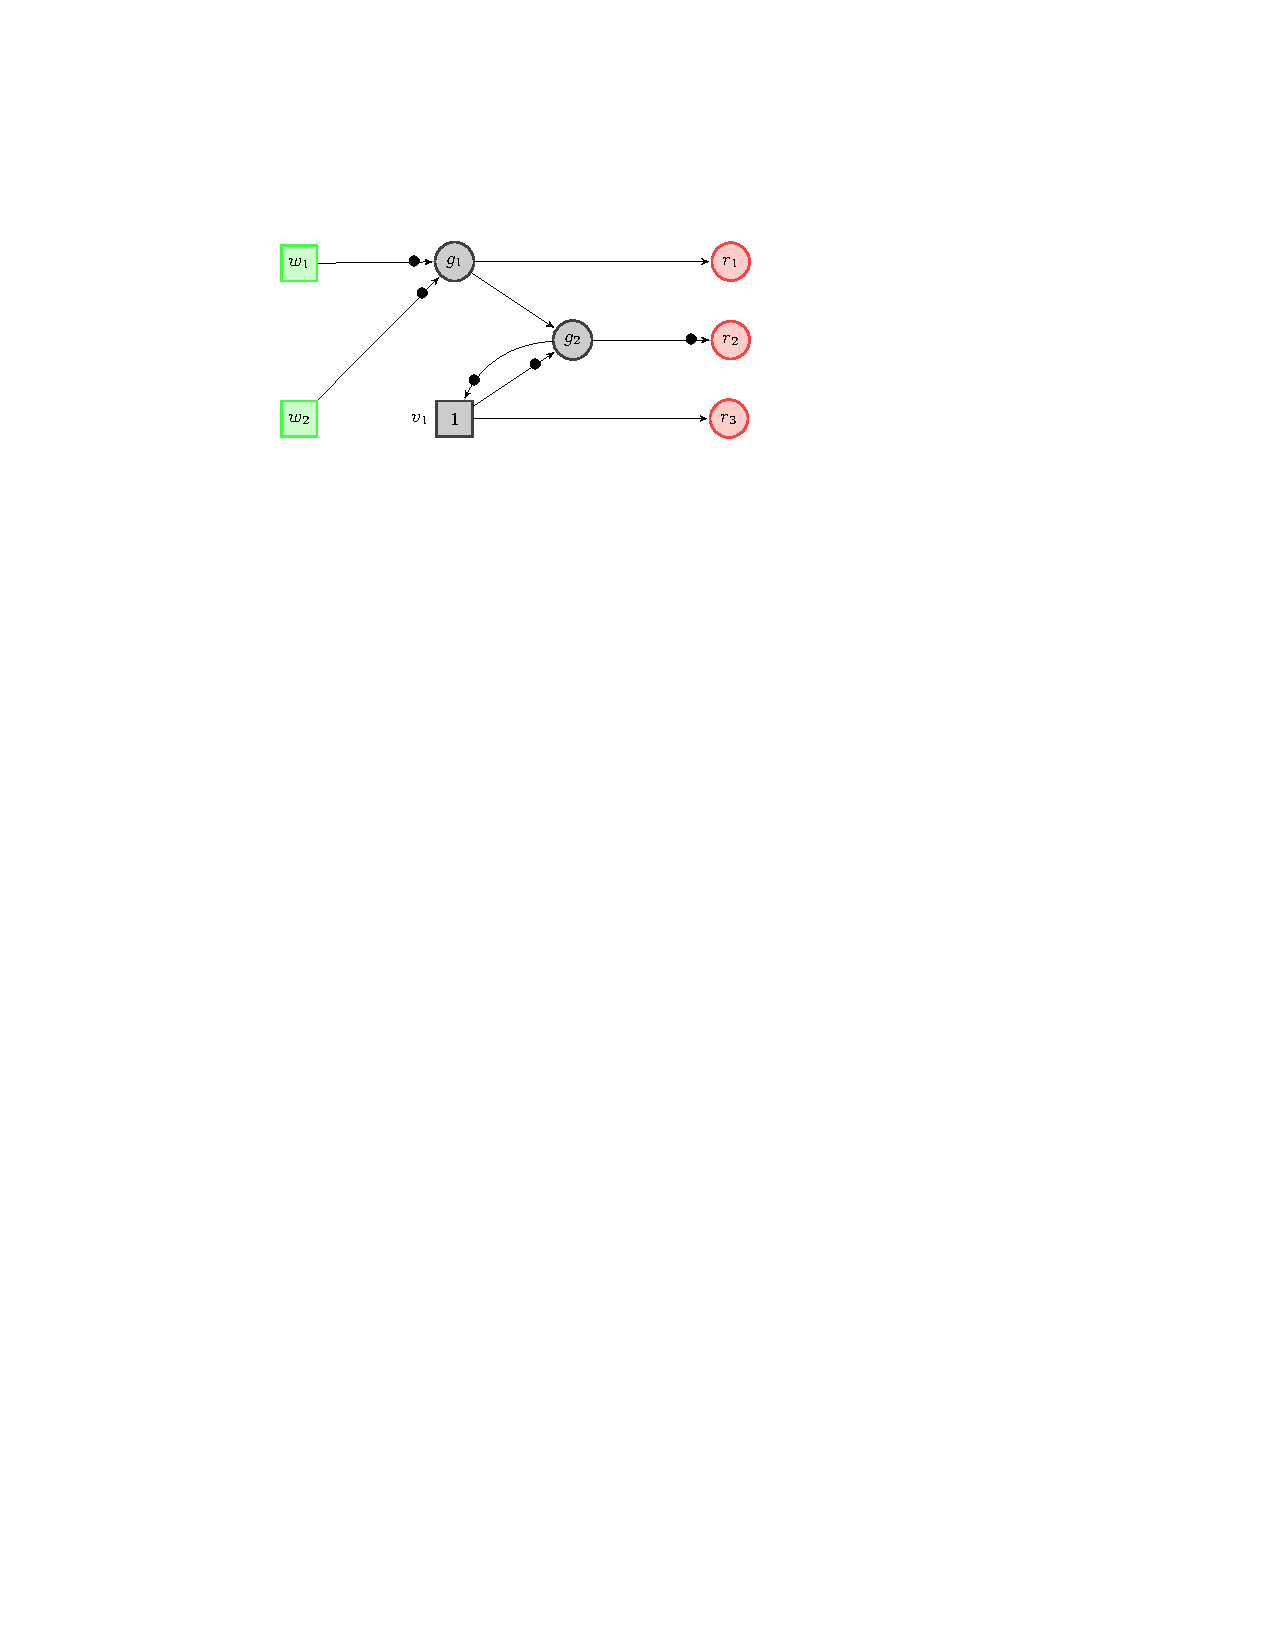
\includegraphics[width=\textwidth]{Example.pdf}
\end{framed}
\caption{\textbf{Left:} And-inverter graph describing a system with two
inputs $w_1$ and $w_2$ (green boxes), one latch $v_1$ with initial value 1 (grey box), two gates $g_1$ and $g_2$ (gray circles), and three invariant requirements $r_1=\Always g_1$, $r_2=\Always \lnot g_2$ and $r_3=\Always v_1$ (red circles). 
The arrows represent logical dependencies, and bullets in the arrows imply negation.}
\label{fig:Preliminaries:AIGExample}
\end{figure}
    %
The set states for this system is $\vect{V}=2^{\set{v_1}}$, the inputs are $\vect{W}=2^{\set{w_1,w_2}}$
%\set{\!\AsSequence{(w_1,0),(w_2,0)},\AsSequence{(w_1,0),(w_2,1)},\AsSequence{(w_1,1),(w_2,0)},\AsSequence{(w_1,1),(w_2,1)}\!}$
, and the initial state is $\vect{v}(0)$, where $\vec{v}(0)[v_1]=1$.

For this example, we define three requirements: $r_1\triangleq\Always g_1$, $r_2 \triangleq\Always \lnot g_2$, and $r_3\triangleq\Always v_1$. This system satisfies $r_2$ and $r_3$, but it fails $r_1$ because $w_1=1$ and $w_2=0$ results in $g_1(0)$ being 0.

In Example~\ref{ex:simple}, the COI for the requirements are $\blacktriangledown(\Always g_1)=\set{g_1,w_1,w_2}$, and $\blacktriangledown(\Always g_2)=\blacktriangledown(\Always g_3)=\set{g_1,g_2,v_1,w_1,w_2}$.
\end{example}
The set of \emph{sources} of an expression $e\in E$, denoted $\mathtt{src}(e)$ is the set of latches and inputs in the COI of $e$; formally, $\mathtt{src}(e)\triangleq \blacktriangledown(e) \cap (V \cup W)$. The \emph{Jaccard index} of two expressions $e_1$ and $e_2$ is equal to $
\frac{|\mathtt{src}(e_1)\cap \mathtt{src}(e_2)|}{|\mathtt{src}(e_1)\cup\mathtt{src}(e_2)|}
$. This index provides a measure of how similar the sources of $e_1$ and $e_2$ are. 

The \emph{dual cone-of-influence} (IOC) of a component $c \in C$, denoted $\blacktriangle(c)$, is the set of components influenced by $c$; more precisely 
$\blacktriangle(c) \triangleq \set{c' \in  C | c\in \blacktriangledown(c')}.$


\section{Cyber-Physical System} 
\todo[inline]{This section probably makes more sense in its own chapter, when we explain what the latent behaviour of a CPS is.}
\section{Side Channels}